\section{Instalasi Android Studio}
Sebelum mengedit alangkah baiknya diinstall terlebih dahulu editornya seperti sebagai berikut :
\begin{enumerate}
	\item Download installernya terlebih dahulu berikut linknya :
\par https://developer.android.com/studio?hl=id.
	\item \textit{Double-click} pada tulisan download android studio pada gambar \ref{fig:installer}
		 \begin{figure}[!htbp]
  		 \centering
 		 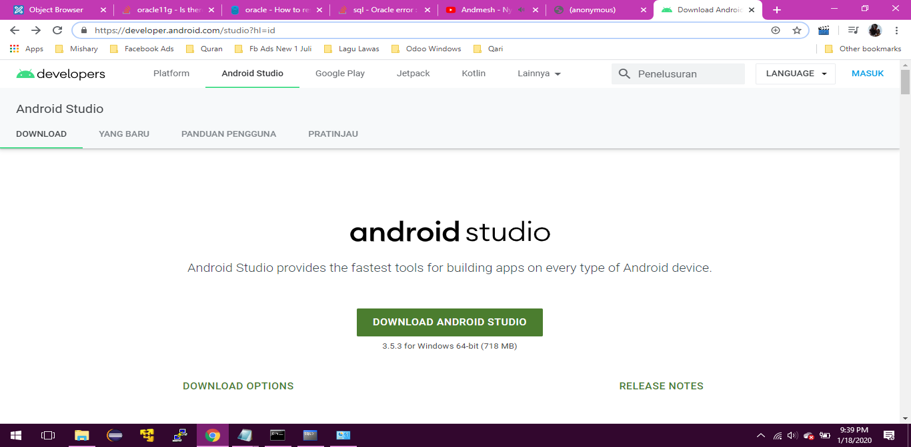
\includegraphics[width=.75\textwidth]{figures/In1.png}
  		 \caption{Ini adalah langkah pertama untuk install Android Studio, buka website resmi Android Studio}\label{fig:installer}
		 \end{figure}
	\item Maka akan muncul halaman awal installer seperti pada gambar  \ref{fig:agreement}
		 \begin{figure}[!htbp]
  		 \centering
 		 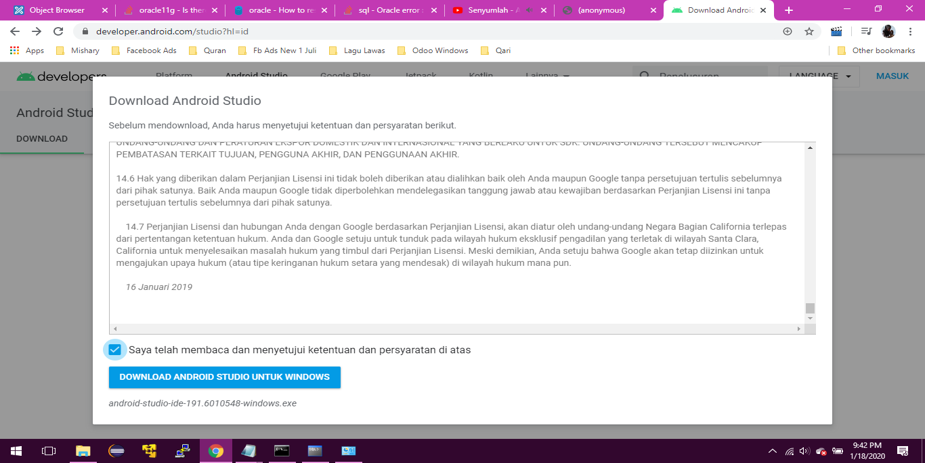
\includegraphics[width=.75\textwidth]{figures/In2.png}
  		 \caption{Ini adalah Halaman persetujuan install}\label{fig:agreement}
		 \end{figure}
	\item Klik \textit{Next} maka akan muncul Halaman installasi scope seperti pada gambar \ref{fig:IS}
		 \begin{figure}[!htbp]
  		 \centering
 		 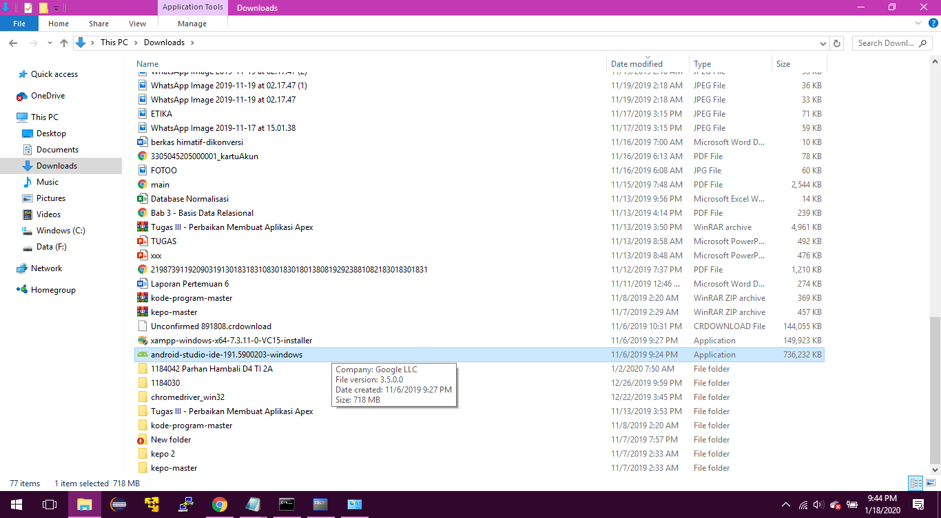
\includegraphics[width=.75\textwidth]{figures/In3.png}
  		 \caption{Ini adalah Halaman istallasi scope}\label{fig:IS}
		 \end{figure}
	\item Klik \textit{Next} maka akan muncul Halaman dari tampilan Android Studio seperti pada gambar \ref{fig:paper}
		 \begin{figure}[!htbp]
  		 \centering
 		 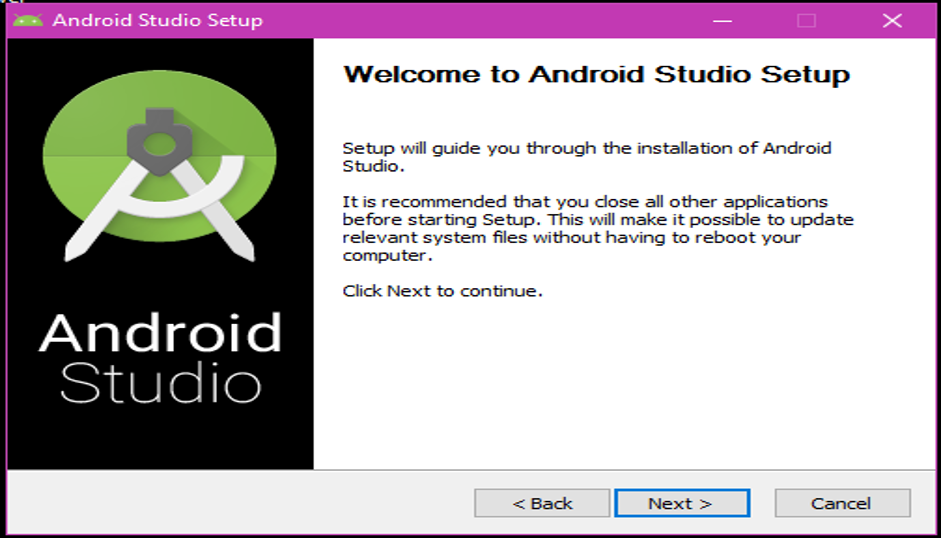
\includegraphics[width=.75\textwidth]{figures/In4.png}
  		 \caption{Ini adalah Halaman penentuan ukuran kertas}\label{fig:paper}
		 \end{figure}
	\item Klik \textit{Next} untuk melanjutkan proses intalasi \ref{fig:dir}
		 \begin{figure}[!htbp]
  		 \centering
 		 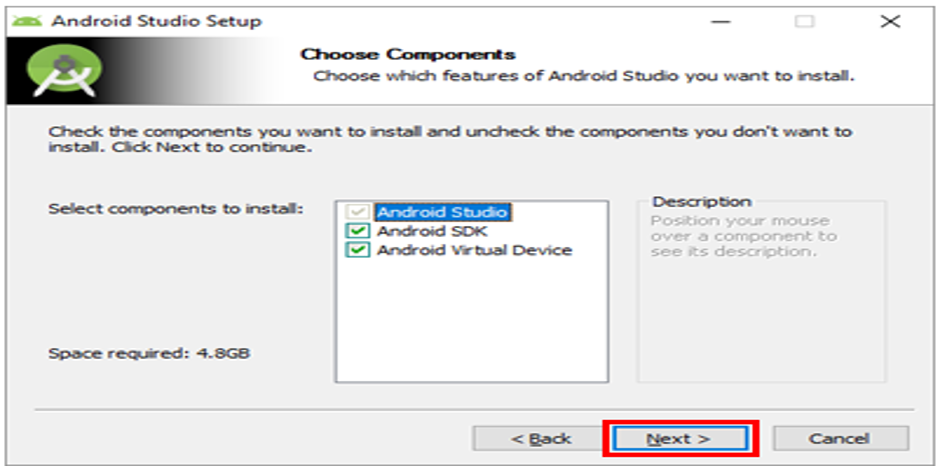
\includegraphics[width=.75\textwidth]{figures/In5.png}
  		 \caption{Ini adalah Halaman Welcome Android Studio}\label{fig:dir}
		 \end{figure}
	\item Klik \textit{Next} maka akan muncul halaman untuk memulai proses install seperti pada gambar \ref{fig:start}
		 \begin{figure}[!htbp]
  		 \centering
 		 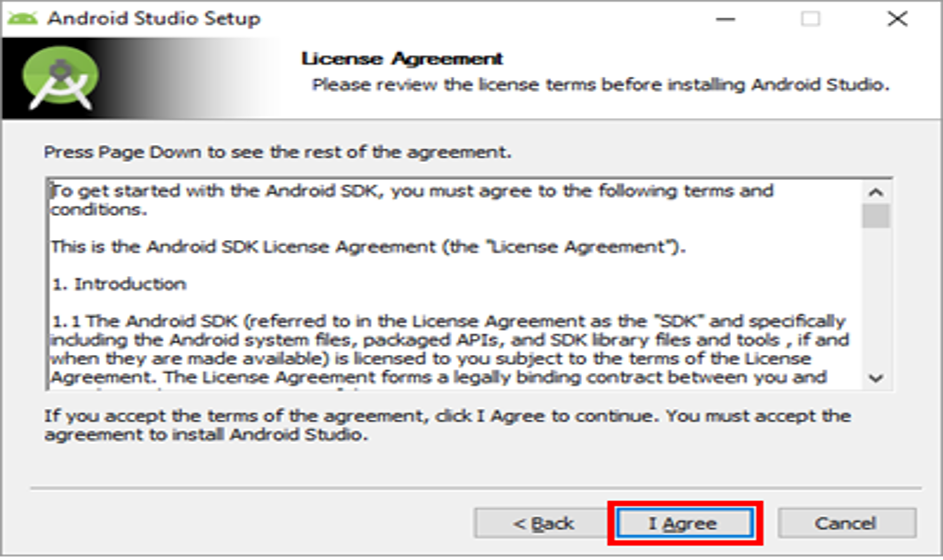
\includegraphics[width=.75\textwidth]{figures/In6.png}
  		 \caption{Ini adalah Halaman memulai install dengan memilih componen Android Studio}\label{fig:start}
		 \end{figure}
	\item Klik \textit{Start} maka proses installasi akan dimulai seperti pada gambar \ref{fig:proses}
		 \begin{figure}[!htbp]
  		 \centering
 		 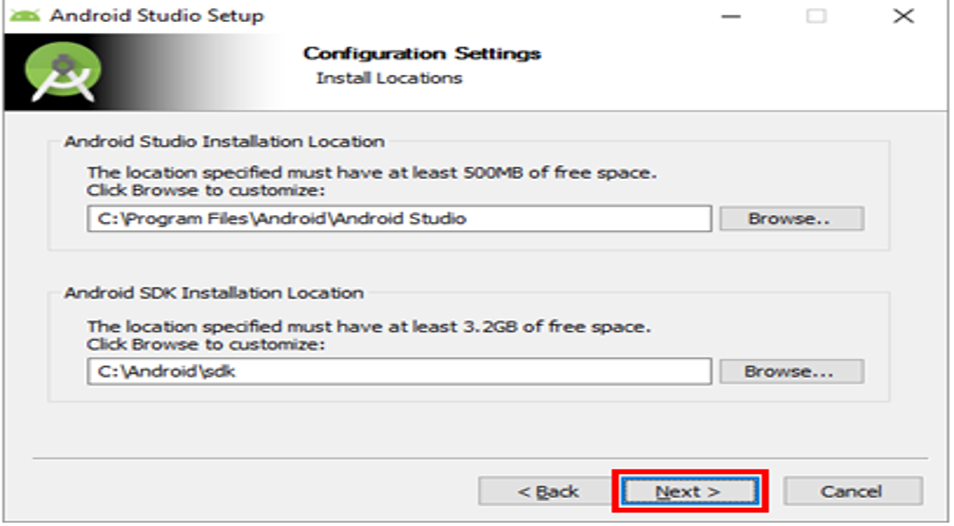
\includegraphics[width=.75\textwidth]{figures/In7.png}
  		 \caption{Ini adalah Proses installasi unutk persetujuan Androis SDK License Agreement}\label{fig:proses}
		 \end{figure}
	\item  Klik \textit{Next} untuk menentukan lokasi penyimpanan Android Studio \ref{fig:ex}
		 \begin{figure}[!htbp]
  		 \centering
 		 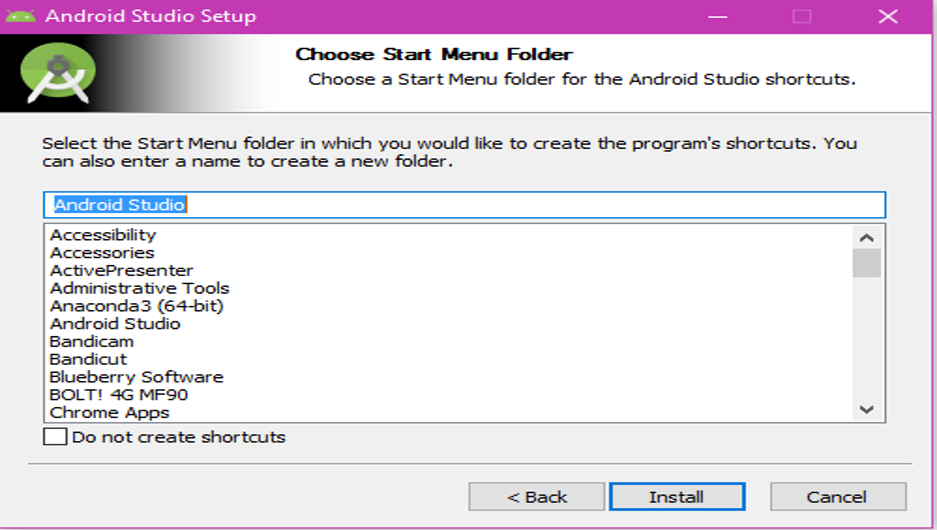
\includegraphics[width=.75\textwidth]{figures/In8.png}
  		 \caption{Ini adalah Halaman untuk penyimpanan Android Studio}\label{fig:ex}
		 \end{figure}
	\item Klik \textit{Install} maka akan muncul halaman seperti pada gambar \ref{fig:done} maka installasi siap untuk dimulai.
		 \begin{figure}[!htbp]
  		 \centering
 		 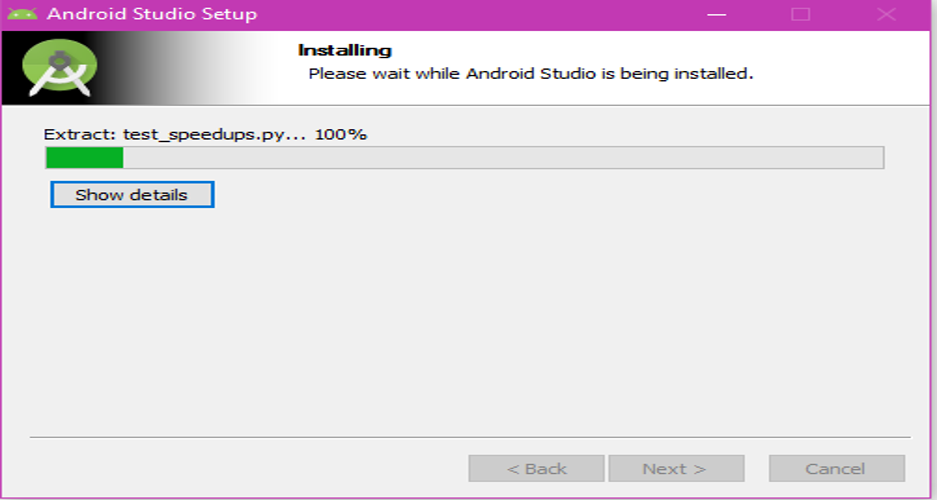
\includegraphics[width=.75\textwidth]{figures/In9.png}
  		 \caption{Installasi segera dimulai}\label{fig:done}
		 \end{figure}
		 \item Klik \textit{Next} maka akan muncul halaman seperti pada gambar \ref{fig:done} maka installasi sedang berjalan, tunggu hingga proses loading berhenti.
		 \begin{figure}[!htbp]
  		 \centering
 		 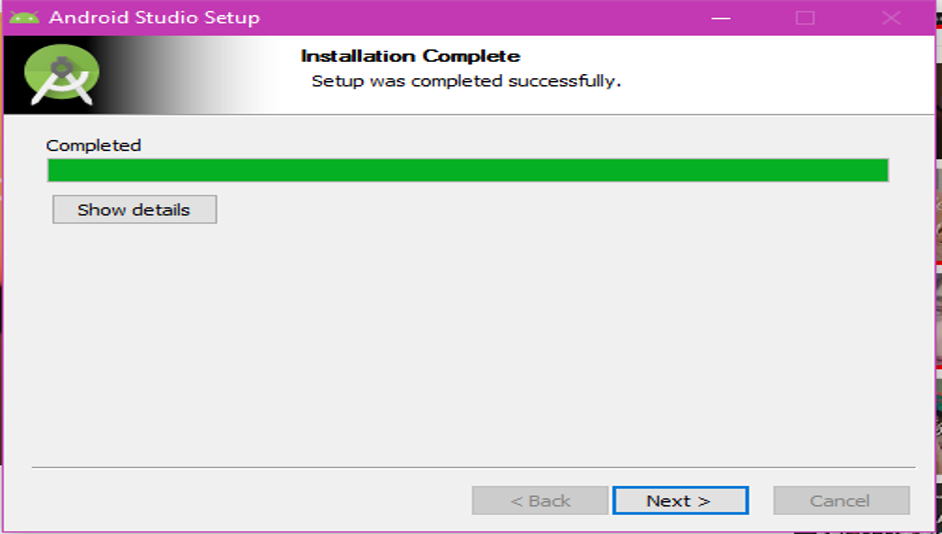
\includegraphics[width=.75\textwidth]{figures/In10.png}
  		 \caption{Installasi sedang berjalan}\label{fig:done}
		 \end{figure}
		 \item Klik \textit{Next} maka akan muncul halaman seperti pada gambar \ref{fig:done} maka installasi siap digunakan.
		 \begin{figure}[!htbp]
  		 \centering
 		 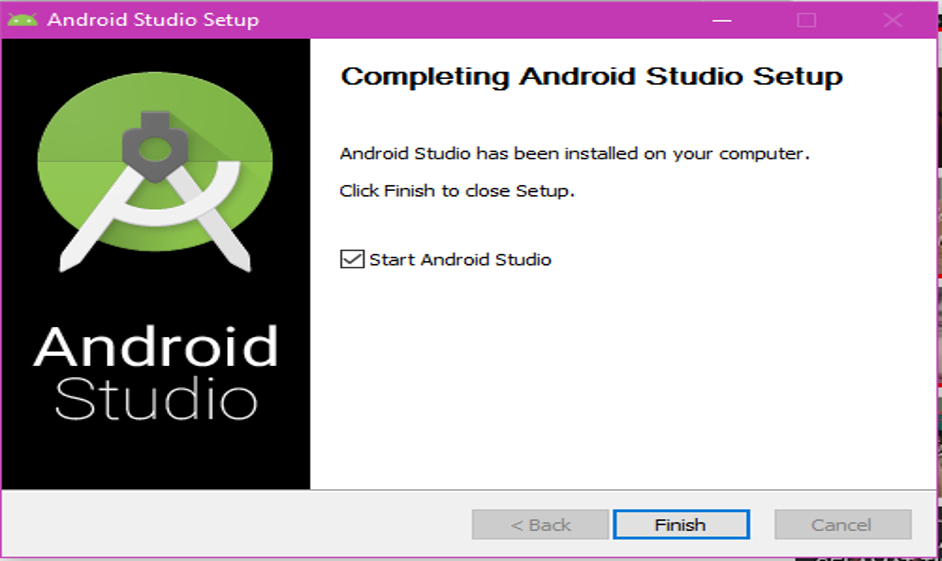
\includegraphics[width=.75\textwidth]{figures/In11.png}
  		 \caption{Installasi sudah selesai}\label{fig:done}
		 \end{figure}
		 \item Klik \textit{Next} maka akan muncul halaman seperti pada gambar \ref{fig:done} maka installasi sudah selesai dilakukan dan program siap digunakan.
		 \begin{figure}[!htbp]
  		 \centering
 		 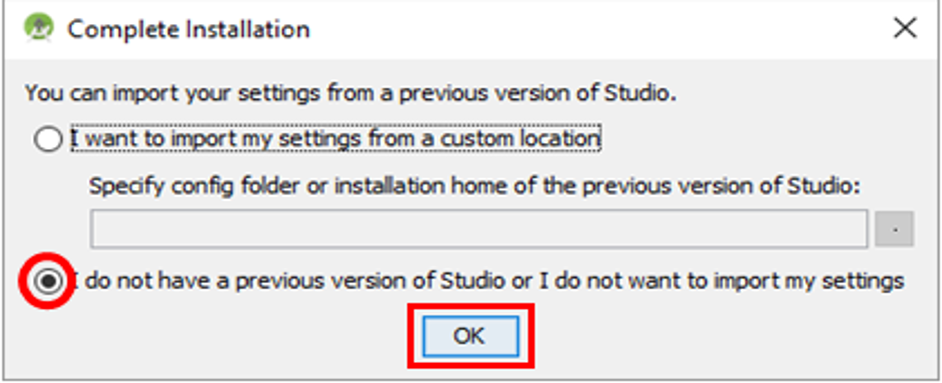
\includegraphics[width=.75\textwidth]{figures/In12.png}
  		 \caption{Installasi sudah selesai}\label{fig:done}
		 \end{figure}
		 \item Klik \textit{Next} maka akan muncul halaman seperti pada gambar \ref{fig:done} disini akan diberikan dua opsi untuk memberikan tanda cheklist pada 2 opsi.
		 \begin{figure}[!htbp]
  		 \centering
 		 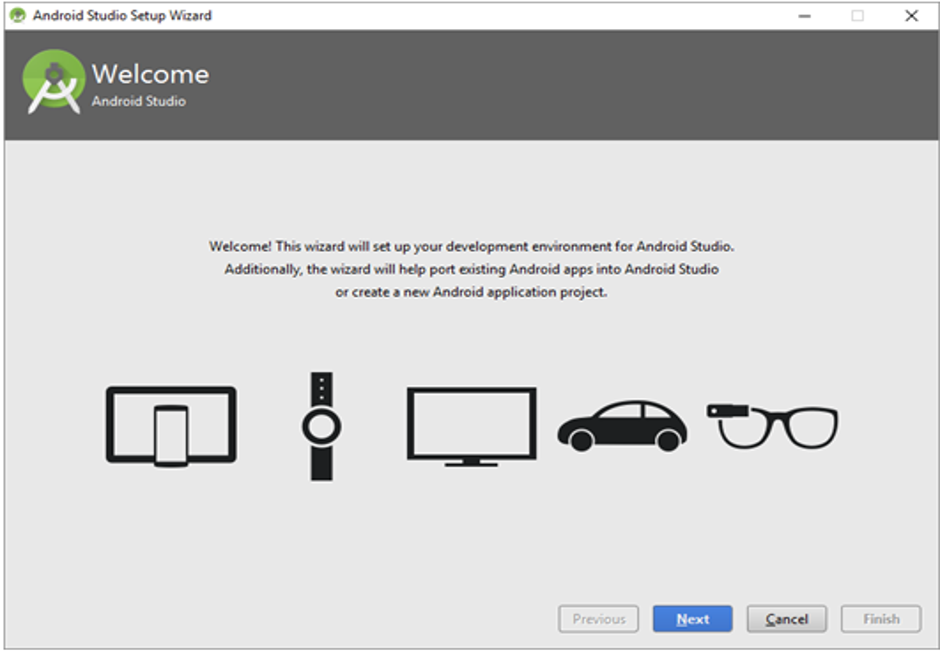
\includegraphics[width=.75\textwidth]{figures/In13.png}
  		 \caption{Pilih untuk yang ada lingkaran merah}\label{fig:done}
		 \end{figure}
		 \item Klik \textit{Next} maka akan muncul halaman seperti pada gambar \ref{fig:done} klik saja next.
		 \begin{figure}[!htbp]
  		 \centering
 		 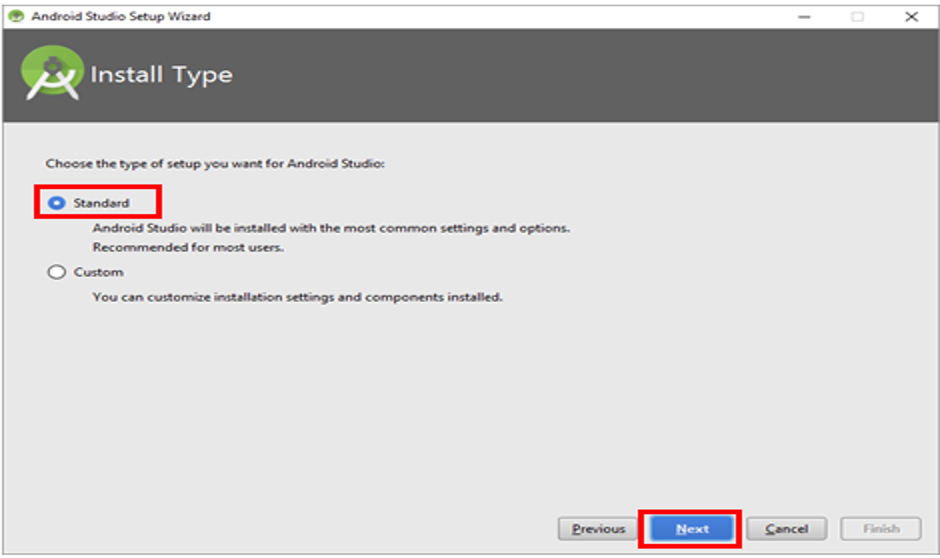
\includegraphics[width=.75\textwidth]{figures/In14.png}
  		 \caption{klik Next}\label{fig:done}
		 \end{figure}
		 \item Klik \textit{Next} maka akan muncul halaman seperti pada gambar \ref{fig:done} maka akan dberikan 2 pilihan tipe untuk Android Studio.
		 \begin{figure}[!htbp]
  		 \centering
 		 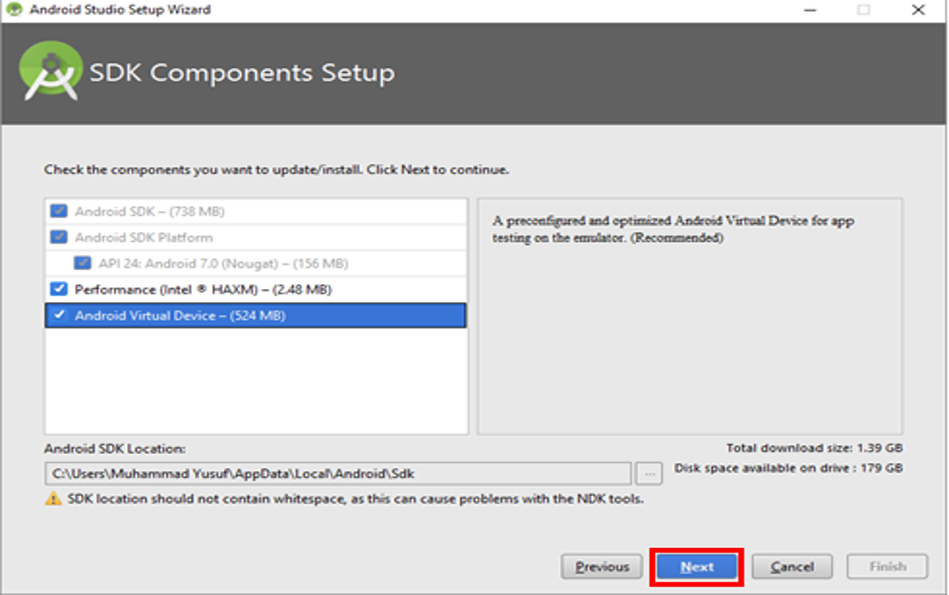
\includegraphics[width=.75\textwidth]{figures/In15.png}
  		 \caption{Pilih yang standard}\label{fig:done}
		 \end{figure}
		 \item Klik \textit{Next} maka akan muncul halaman seperti pada gambar \ref{fig:done} maka pilih yang akan diinstal dan yg dibutuhkan Android Studio
		 \begin{figure}[!htbp]
  		 \centering
 		 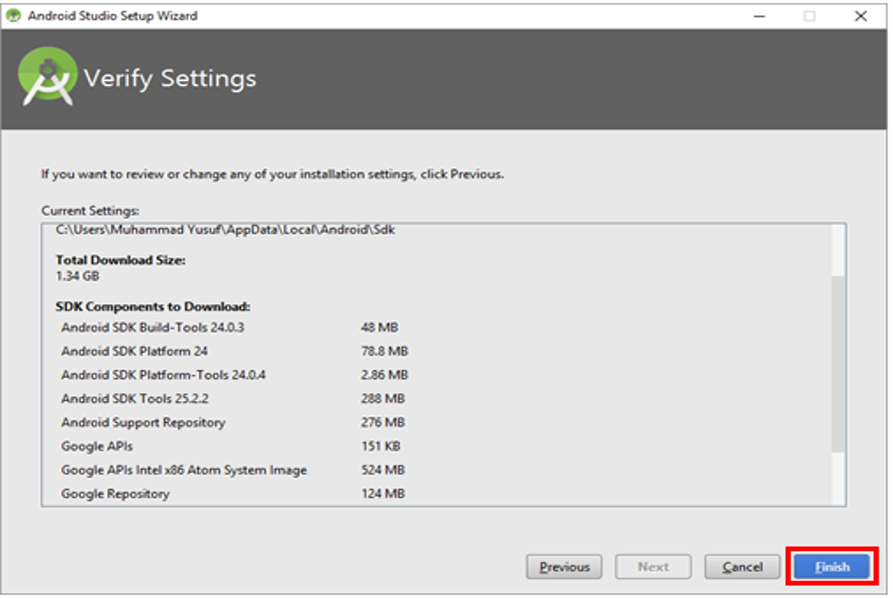
\includegraphics[width=.75\textwidth]{figures/In16.png}
  		 \caption{Pilih sesuai yang ada diatas}\label{fig:done}
		 \end{figure}
		 \item Klik \textit{Next} maka akan muncul halaman seperti pada gambar \ref{fig:done} selanjutnya klik Finsih.
		 \begin{figure}[!htbp]
  		 \centering
 		 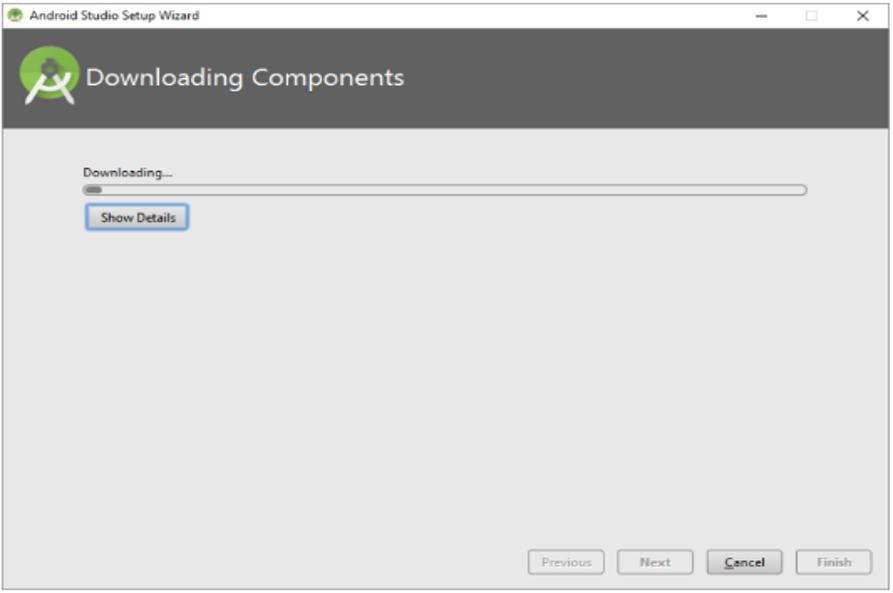
\includegraphics[width=.75\textwidth]{figures/In17.png}
  		 \caption{klik Finsih}\label{fig:done}
		 \end{figure}
		 \item Klik \textit{Next} maka akan muncul halaman seperti pada gambar \ref{fig:done} tunggu hingga proses downloading selesai.
		 \begin{figure}[!htbp]
  		 \centering
 		 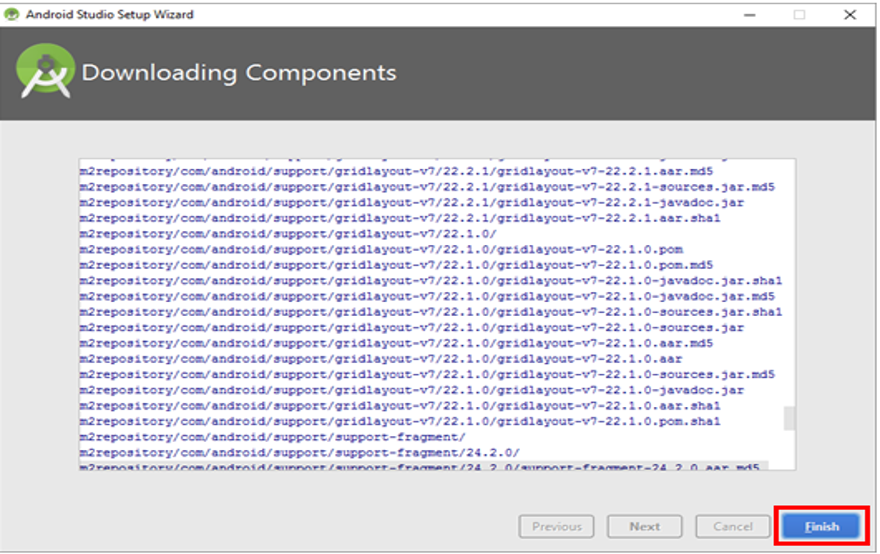
\includegraphics[width=.75\textwidth]{figures/In18.png}
  		 \caption{Tunggu proses downloadng}\label{fig:done}
		 \end{figure}
		 \item Klik \textit{Next} maka akan muncul halaman seperti pada gambar \ref{fig:done} maka installasi sudah selesai dilakukan.
		 \begin{figure}[!htbp]
  		 \centering
 		 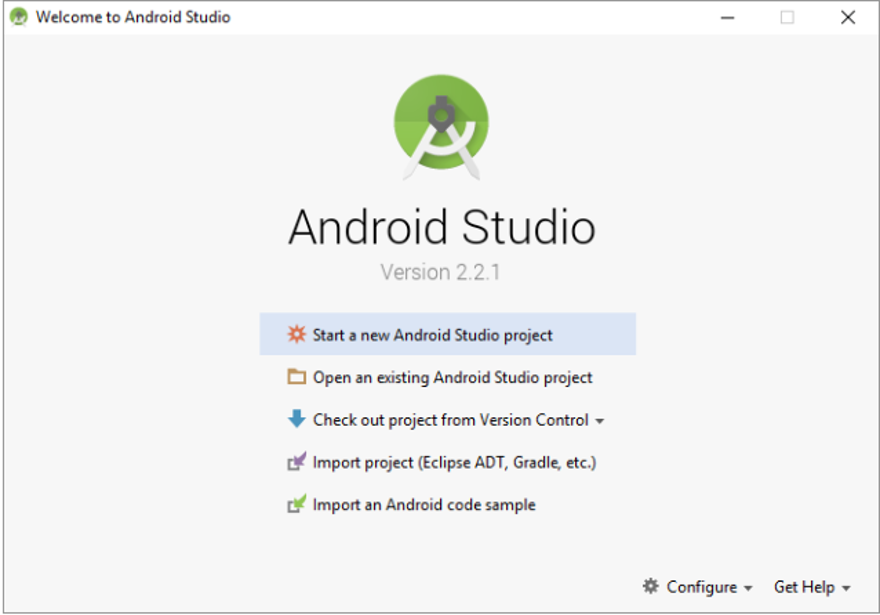
\includegraphics[width=.75\textwidth]{figures/In19.png}
  		 \caption{Installasi sudah selesai}\label{fig:done}
		 \end{figure}
		 \item Klik \textit{Next} maka akan muncul halaman seperti pada gambar \ref{fig:done} maka installasi sudah siap digunakan.
		 \begin{figure}[!htbp]
  		 \centering
 		 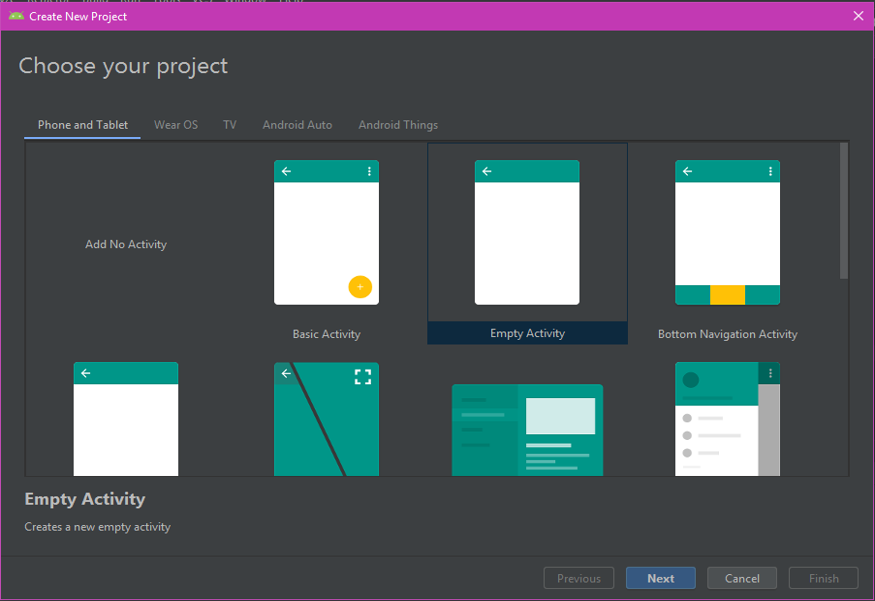
\includegraphics[width=.75\textwidth]{figures/In20.png}
  		 \caption{Andrid Studio siap digunakan}\label{fig:done}
		 \end{figure}
\end{enumerate}
